\documentclass[10pt, a4paper,twocolumn, oneside]{book}
\usepackage[T1]{fontenc}
\usepackage{fancyhdr}
%\usepackage{ps4pdf}
\pagestyle{fancyplain}
\usepackage[pdftex]{graphicx}
\graphicspath{ {./images/} }
\usepackage{lscape}
\usepackage{pdflscape}
\usepackage{amsmath}
\usepackage{booktabs}
\usepackage{multirow}
\usepackage{nicefrac}
\usepackage{makecell}
\usepackage{imakeidx}
\usepackage{enumitem}
\usepackage[margin=0.7in]{geometry}
\usepackage[table]{xcolor}
\usepackage{amsmath}
\usepackage{hyperref}

\pagecolor{black}
\definecolor{lightgray}{gray}{0.2}
\definecolor{darkgray}{gray}{0.8}
\color{darkgray}


%\usepackage{fetamont}
%\usepackage[T1]{fontenc}
\makeindex[columns=3, title=Alphabetical Index,intoc]

\newcommand{\tabitem}{~~\llap{\textbullet}~~}

% \makeatletter
% \renewcommand{\paragraph}{
%   \@startsection{paragraph}{4}{\z@}%
%   {-3.25ex\@plus -1ex \@minus -.2ex}%
%   {0.5ex \@plus .2ex}%
%   {\normalfont\normalsize\bfseries}}
% \makeatother

\renewcommand{\familydefault}{\sfdefault}

\title{Pink Trenchcoat \\ \small{a cyberpunk rule-set}}
\author{Serbitar}

\begin{document}

\maketitle

\tableofcontents

%\begin{abstract}

% \end{abstract}
\chapter{Basics}

This chapter will cover the basics of Pink Trenchcoat including standard RPG
nomenclature as wells as methods of conflict resolution. The rule system
uses a fixed set of resolution methods, which are covered here, that will be used
throughout the system exclusively.

\section{Definitions}

A couple of basic descriptions and definitions are given here.
Throughout the book everything that is a game term with a defined meaning in the
game is written in \textit{italics}, and in upper-case if it is a noun.
All game terms should be found in the index at the end of the book.

\subsection{Gamers}

Everyone that is taking part in the game is a \emph{Gamer}.

\paragraph{Game Master}
\index{Game Master}
\index{GM}

The \emph{Game Master} is the person that is not playing their own \emph{Character},
but all the \emph{Characters} that are not being played by a \emph{Player}.

\paragraph{Players}
\index{Player}
A Player is a \emph{Gamer} that is only playing their \emph{Character} and maybe
\emph{Characters} that are closely connected to this \emph{Character} like
\emph{Drones}, \emph{Agents} or \emph{Contacts}.

\subsection{Characters}

A \emph{Character} is an entity that can actively make decisions in the game world
and act on those decisions. In Pink Trenchcoat this includes (Meta)-Humans, but also
\emph{Agents}, \emph{Drones}, \emph{Spirits} and more.

\paragraph{Player Characters}
\index{Player Character}
\index{PC}

A \emph{Player Characters} or \emph{PC} is a \emph{Character} that is directly and often
exclusively controlled by a \emph{Player}.

\paragraph{Non-Player Characters}
\index{Non-Player Character}
\index{NPC}

All \emph{Non-Player Characters} or \emph{NPC} are most often controlled by the \emph{Game Master}.

\subsection{Mathematics}

Pink Trenchcoat`s resolution system only uses integers. Although during calculation
a number mit be not an integer, it needs to be rounded to the next integer for any
kind of \emph{Test}.

\paragraph{Rounding}
\index{Rounding}

Fractions are always rounded mathematically correct. This means that 0.5 is
rounded to 1.

\section{Dice}
\index{dice}

Like most game systems Pink Trenchcoat uses dice to act as a randomizer for
\emph{Tests}. This is done to increase tension during the game session and include
a random element so that players can not plan everything in advance with 100\%
certainty. However, if the gaming group so chooses, the rule set can be used
completely without dice, as the average result of a die roll is always 0.

Pink Trenchcoat uses five six-sided dice with two “-”, two blank and two “+”
symbols also known as FUDGE dice. They are always used together and there are no
other dice rolls used.


Almost always a player will roll only 5 dice,
and the game master will secretly roll the other 5 dice, either because its
an \emph{Opposed Test}, and the game master is performing the roll for the
opposition, or because it is not an \emph{Opposed Test} and the game master will
roll 5 dice because the player should not be sure of the outcome. Only in cases where
the player is managing the situation fully they should roll the full 10 dice, but
either roll 5 dice twice or use differently coloured dice to calculate
\emph{Criticals} and other functionality the dice roll is covering.

Every test requires 10 dice to be rolled in total.

\hfill

In this rule set, 5 FUDGE dice will always be referred to as: \[\textit{5f}\]
\index{5f}
while the full 10 FUDGE dice will always be referred to as: \[\textit{10f}\]
\index{10f}

\subsection{Result}

The Result of \emph{10f} is calculated by rolling 2 times 5 dice and summing all
“+” as 1 and all “-” as -1 while blanks count as 0.

If the Result of a \emph{10f}roll needs to be calculated in this rule system it will
be denoted as: \[\textit{10fR}\]
\index{10fR}

\paragraph{Probability Distribution}

The average \emph{Result} of any dice roll in Pink Trenchcoat is always 0.
The number of total dice rolled is also always 10 (although, sometimes,
the dice are rolled by different people for psychological reasons, mathematically
this makes no difference).

Using 10 dice, the following statistics apply the outcome of \emph{10fR}.

\subparagraph{Probability for exactly rolling a value}

Sometimes it is good to know what the probabilities to exactly roll a  value are.
The probability distribution of the \emph{10fR} is a gaussian with mean of 0 and
a standard deviation of about 2.6.

\begin{figure}[htb]
    \caption{\emph{10fR} Probability Distribution}
    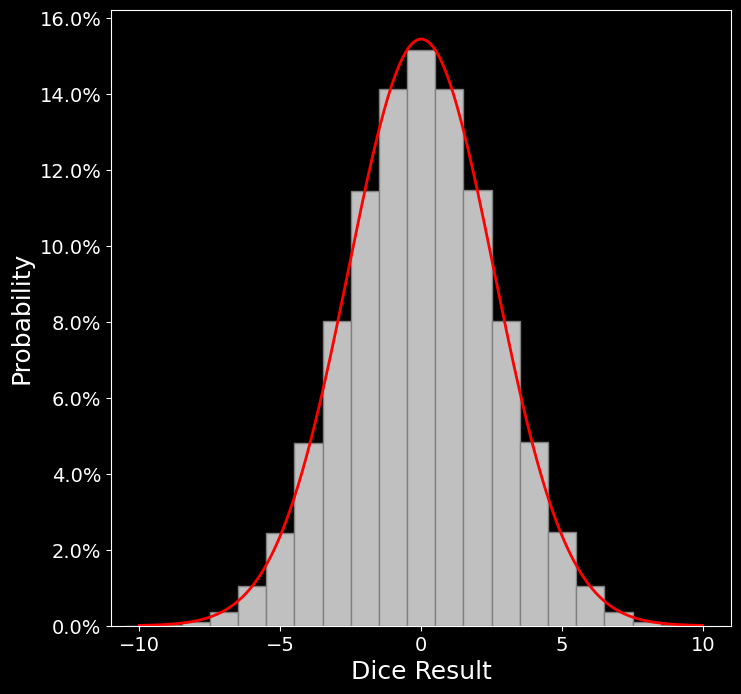
\includegraphics[width=0.95\columnwidth]{10fR}
\end{figure}

\begin{table}[htb]
    \rowcolors{1}{}{lightgray}
    \caption[10fR Probabilities]{10fR Probabilities}
    \label{tab:10fR probabilities}
    \centering
    \begin{tabular}{ccc}
        \toprule
        \textbf{Roll exactly} & \textbf{Chance} & \textbf{one in} \\
        \midrule
        -10/10                & 0.0014\%        & 71000           \\
        -9/9                  & 0.016\%         & 6100            \\
        -8/8                  & 0.088\%         & 1100            \\
        -7/7                  & 0.36\%          & 280             \\
        -6/6                  & 1.0\%           & 96              \\
        -5/5                  & 2.4\%           & 41              \\
        -4/4                  & 4.8\%           & 21              \\
        -3/3                  & 8.0\%           & 13              \\
        -2/2                  & 12\%            & 8.7             \\
        -1/1                  & 14\%            & 7.1             \\
        0                     & 15\%            & 6.6             \\
        \bottomrule
    \end{tabular}
\end{table}

\subparagraph{Probability for rolling a value and lower/higher}


Most of the time it is important to know the probability to at at least a certain
number or higher, or the inverse, the chance to roll a certain number or lower.
Both are important to judge if a \emph{Test} will fail or succeed.

As a rule of thumb, rolling below -5 or above 5 is not happening often. This also
means that \emph{Tests} that only fail when a value smaller than -5 is rolled should
only be done if the success or how well it succeeded or failed is critical for the game.
Instead it can just be assumed that the \emph{Test} succeeded normally.

\begin{figure}[htb]
    \caption{\emph{10fR} Cumulative Probability Distribution}
    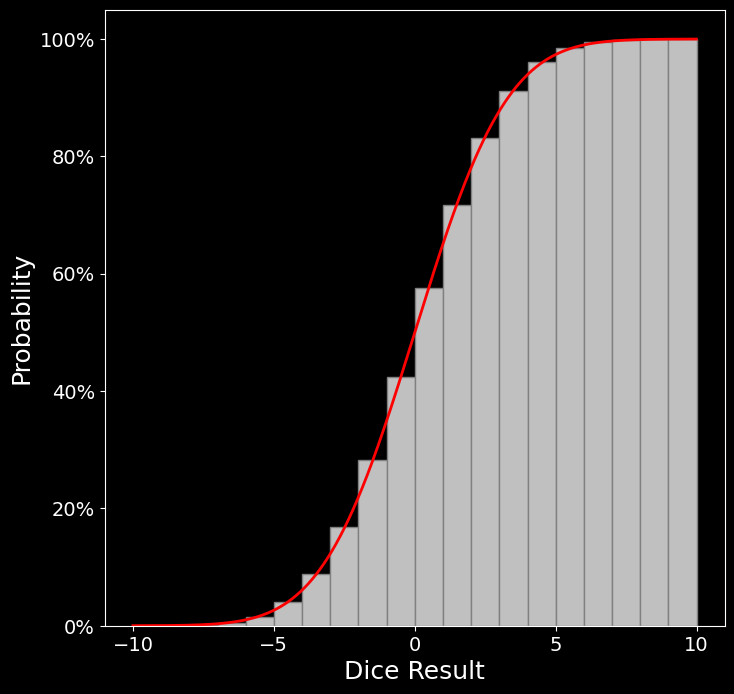
\includegraphics[width=0.95\columnwidth]{10fR_cum}
\end{figure}

\begin{table}[htb]
    \rowcolors{1}{}{lightgray}
    \caption[10fR Cumulative Probabilities]{10fR Cumulative Probabilities}
    \label{tab:10fR cumulative probabilities}
    \centering
    \begin{tabular}{cccc}
        \toprule
        \multicolumn{2}{c}{\textbf{Roll exactly or}} & \multirow{2}{*}{\textbf{Chance}} & \multirow{2}{*}{\textbf{one in}}         \\
        \cmidrule{1-2}
        \textbf{bigger}                              & \textbf{smaller}                 &                                  &       \\
        \midrule
        10                                           & -10                              & 0.0014\%                         & 71000 \\
        9                                            & -9                               & 0.08\%                           & 5600  \\
        8                                            & -8                               & 0.11\%                           & 940   \\
        7                                            & -7                               & 0.46\%                           & 220   \\
        6                                            & -6                               & 1.5\&                            & 66    \\
        5                                            & -5                               & 3.9\%                            & 25    \\
        4                                            & -4                               & 8.8\%                            & 11    \\
        3                                            & -3                               & 17\%                             & 6.0   \\
        2                                            & -2                               & 28\%                             & 3.5   \\
        1                                            & -1                               & 42\%                             & 2.4   \\
        0                                            & 0                                & 58\%                             & 1.7   \\
        \bottomrule
    \end{tabular}
\end{table}

\subsection{Anomalies and Criticals}

The \emph{Result} is not the only quantity that the dice deliver. Another one is
Anomalies and Criticals. They are in principle the same thing, but Criticals are
much more seldom and extreme in their effect.

Criticals and Anomalies are determined only looking at the \emph{5f} roll of either
the player and the game master. This means that both parties in an \emph{Opposed Test}
can generate a Critical or Anomaly at the same time. They happen if multiple dice
show similar symbols.

\paragraph{Anomaly}
\index{Anomaly}
To determine Anomalies the number of similar symbols have to be counted. Every time
4 dice of a \emph{5f} roll show the same symbol, an Anomaly happened.
This can be four ''+'' (Positive Anomaly), four ''-'' (Negative Anomaly) or four
blanks (Neutral Anomaly).

The chance to roll an Anomaly is 4.1\% for any kind of Anomaly. This means that the
chance is 12.3\% to have any kind of Anomaly in a \emph{Test}. The Game Master
needs to decide whether they want to ignore \emph{Anomalies} in an
\emph{Opposing Test}, if the opposing faction is an NPC. The same applies for the other \emph{5f} that are
rolled in a \emph{Unopposed Test}.

\subparagraph{Positive and Negative Anomaly}
\index{Positiv Anomaly}
\index{Negative Anomaly}
The result of a positive or negative Anomaly enhances the outcome of the
\emph{Test} in a positive or negative way respectively, but does not change the
\emph{Result}. The Game Master needs to look at the situation and think of any
positive or negative effects that could happen.

This includes:
\begin{itemize}[parsep=0em]
    \item Taking more/less time of an action in combat that normally can not
          be slowed/sped up
    \item getting into a advantageous/disadvantageous position when performing a
          melee attack
    \item increasing/decreasing connection status of a contact when doing legwork
    \item using less/more resources when crafting an item
\end{itemize}

\subparagraph{Neutral Anomaly}
\index{Neutral Anomaly}
A neutral Moderate Critical should just create unusual side effects to an outcome.
Again the Game Master should be free to invent anything coming to their mind.

For example:
\begin{itemize}[parsep=0em]
    \item A
    \item b
    \item c
\end{itemize}

\paragraph{Critical}
\index{Critical}
Criticals happens if all 5 dice of a \emph{5f} show the same symbol. As with Anomalies
there are positive, negative and neutral Criticals. Both the chance and the effect of
a Critical are much more radical than an Anomaly.

The chance to roll any kind of Critical is 0.4\%.

\subparagraph{Positive Critical}
\index{Positive Critical}

If there is a remote chance of the \emph{Test} succeeding, it will. This does not
allow \emph{PC} to do things that are impossible like surviving an atomic blast or
succeeding in a wrestling match with a dragon, but anything close to that.

\subparagraph{Negative Critical}
\index{Negative Critical}

The \emph{Test} fails and it fails spectacularly. The Game Master is free to invent
any convenient explanations. There is always a way something can fail.

\subparagraph{Neutral Critical}
\index{Neutral Critical}

The \emph{Result} of the \emph{Test} is not affected, but something very strange
happens. The Game Master can do whatever they see fit.


\subsection{Non Blanks}

The Non Blanks of \emph{5f}is calculated by counting all the ''+'' and ''-''
symbols, resulting in a number from 0 to 5.

If the Non Blanks need to be calculated from a \emph{Test} this is denoted as:
\[ \textit{5fN} \]
\index{5fN}
Note that does not mean that an additional \emph{5f}need to be rolled in addition to
the \emph{10f} of the \emph{Test} itself, but instead use the \emph{5f}from the
existing \emph{10f}roll.

The Non Blanks are used for various secondary purposes of a dice roll.

\begin{figure}[htb]
    \caption{\emph{5fN} Probability Distribution}
    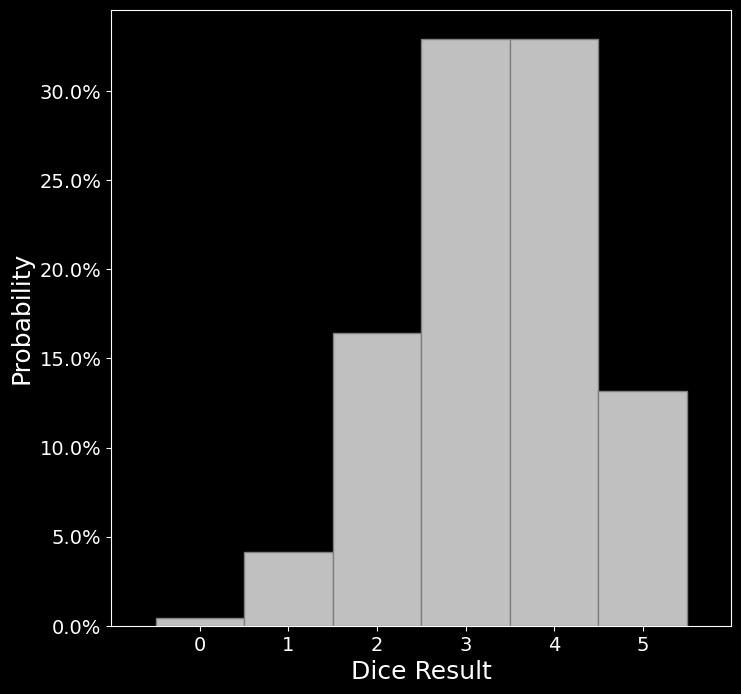
\includegraphics[width=0.95\columnwidth]{5fN}
\end{figure}

\begin{table}[htb]
    \rowcolors{1}{}{lightgray}
    \caption[5dN Probabilities]{5dN Probabilities}
    \label{tab:5dN probabilities}
    \centering
    \begin{tabular}{ccc}
        \toprule
        \textbf{Roll exactly} & \textbf{Chance} & \textbf{one in} \\
        \midrule
        5                     & 13\%            & 7.6             \\
        4                     & 33\%            & 3.0             \\
        3                     & 33\%            & 3.0             \\
        2                     & 16\%            & 6.1             \\
        1                     & 4.1\%           & 24              \\
        0                     & 0.4\%           & 240             \\
        \bottomrule
    \end{tabular}
\end{table}

\section{Tests}
\index{Test}

A test determines the outcome of a certain action, which has a certain probability to
fail and which has an important impact on the game session if it fails. Tests should
not be rolled if it is clear that the test will succeed, like in the case of opening
a door. Tests should also not be rolled if the result is irrelevant for the game
session, like when a character is trying to beat a popular game in their spare time.

Every time the outcome of an action is, given the capabilities of the acting
character, in doubt, or if the result needs to be quantified, a \emph{Test} is rolled.

\subsection{Test Anatomy}

All Tests in Pink Trenchcoat look like the following:

\begin{equation}
    \begin{split}
        \textit{Test Quality} = {} & \textit{10fR}  + \textit{Ability Score(s)} \\
        & + \textit{Modifiers(s)}
    \end{split}
\end{equation}


The \emph{10fR} was already explained in the previous section.

\paragraph{Ability Score}
\index{Ability Score}

The Ability Score is a number giving the proficiency of the person or entity that
performs the \emph{Test} to achieve the result. The higher, the better.

Normally Ability Scores are either \emph{Attributes} or \emph{Skills} of a character.

\subparagraph{Limits}
\index{Limit}

Sometimes tools and other situational effects are not modeled as a \emph{Modifier}
that is added or subtracted but as a \emph{Limit} to the \emph{Ability Score}. In
case the \emph{Ability Score} can not be higher than the \emph{Limit}.

\emph{Limits} to the \emph{Ability Score} are noted as follows:

\begin{equation}
    \textit{Ability Score}(\textit{Limit})
\end{equation}

\paragraph{Modifier}

\emph{Modifier} can be anything from a threshold that needs to be achieved to
circumstantial \emph{Modifiers} like visual conditions, tools or wounds that can
change the result of a \emph{Test}. If a \emph{Modifier} is helping the
\emph{Character} performing the \emph{Test}, like good tools, or support from friends,
it is positive. If it is an obstacle of problem for the \emph{Character} performing
the \emph{Test}, the \emph{Modifier} is negative.

\paragraph{Test Quality}
\index{Test Quality}
\index{TQ}

The \emph{Test Quality} ot \emph{TQ} is the value that results from adding the
\emph{10fR} the \emph{Ability Score} and the \emph{Modifiers}. If the
\emph{Test Quality} is zero or positive, the \emph{Test} succeed, if it negative
it failed. The higher the \emph{Test Quality} the better the result and the lower
the \emph{Test Quality} the worse the failure.


\begin{table}[htb]
    \rowcolors{1}{}{lightgray}
    \caption[Test Quality]{Test Quality}
    \label{tab:test quality}
    \centering
    \begin{tabular}{cl}
        \toprule
        \textbf{TQ} & \textbf{Description} \\
        \midrule
        < -9        & Epic Fail            \\
        -7 to -9    & Severe Failure       \\
        -4 to -6    & Decisive Failure     \\
        -1 to -3    & Failure              \\
        0           & Barely made it       \\
        1 to 3      & Acceptable           \\
        4 to 6      & Good Result          \\
        7 to 9      & Exceptional          \\
        > 9         & Epic Success         \\
        \bottomrule
    \end{tabular}
\end{table}

\subsection{Unopposed Tests}
\index{Unopposed Test}

In an \emph{Unopposed Tests} a \emph{Character} is not testing against another
\emph{Character} but against the environment. Typical \emph{Unopposed Tests} include:

\begin{itemize}[parsep=0em]
    \item crafting something
    \item climbing a wall
    \item running fast
    \item remembering something
\end{itemize}

In this case, the \emph{Ability Score} is just the relevant value from the
\emph{Character} and the \emph{Modifier} is the difficulty of the task plus any
additional situational \emph{Modifiers}.

This rule system defines the \emph{Ability Scores} to use in an
\emph{Unopposed Test} in the following notation:

\begin{equation}
    \textit{Ability Score}_\textit{Acting Character} \; + \textit{Modifier}
\end{equation}

In case of a climbing test for a given wall, that would be:

\begin{equation*}
    \textit{Climbing} \; -6
\end{equation*}

\subsection{Opposed Tests}
\index{Opposed Test}

If two \emph{Characters} are fighting against each other, either literally in melee
combat or figuratively when one \emph{Character} tries to sneak by and the other to
spot the sneaker, an \emph{Opposed Test} is called for. In this case, both involved
\emph{Characters} \emph{Ability Scores} are used. The definition of the \emph{Test}
explains which values of a \emph{Character} are used, as this can be the same, in the
case of melee combat or be different in the case of sneaking.

This rule system defines the \emph{Ability Scores} to use in an
\emph{Opposed Test} in the following notation:

\begin{equation}
    \textit{Ability Score}_\textit{Attacker} \; \textit{vs.} \; \textit{Ability Score}_\textit{Defender}
\end{equation}

In case of melee combat this would mean:

\begin{equation*}
    \textit{Melee Combat} \; \textit{vs.} \; \textit{Melee Combat}
\end{equation*}

In case of sneaking it would mean:

\begin{equation*}
    \textit{Stealth} \; \textit{vs.} \; \textit{Perception}
\end{equation*}

The final \emph{Test Quality} is then calculated as follows:

\begin{equation}
    \begin{split}
        \textit{Test Quality} = {} & \textit{10fR} \\
        & + \textit{Ability Score}_\textit{Attacker} \\
        & + \textit{Modifiers(s)}_\textit{Attacker} \\
        & - \textit{Ability Score}_\textit{Defender} \\
        & - \textit{Modifiers(s)}_\textit{Defender} \\
    \end{split}
\end{equation}


Ties\index{Ties} are broken either by bespoke tie breakers given in the specific rules section,
or, and if those tie breakers still end in a tie, by the\emph{Game Master}. They
can decide to either flip a coin or decide for themselves.

\subsection{Supported Tests}\index{Supported Test}

If one or more \emph{Characters} are helping another \emph{Character} to do a task
that can not be split into subtasks, but all characters have to do the full task,
this is a \emph{Supported Test}.

\begin{itemize}[parsep=0em]
    \item climbing a wall together
    \item helping a character to sneak
    \item crossing a mine-field
\end{itemize}

In this case the \emph{Ability Score} for the \emph{Supported Test} is the average
\emph{Ability Score} of all the \emph{Characters} involved. The \emph{Modifiers}
for the \emph{Supported Test} are the average
\emph{Modifiers} of all the \emph{Characters} involved -1.

The \emph{Game Master} decides which \emph{Tests} can be supported.

\subsection{Collaborative Tests}
\index{Collaborative Test}

If one or more \emph{Characters} are working together, distributing the work to
perform a task that can be broken down into independent parts this is a
\emph{Team-Play Test}. The goal is to either increase the quality of the result, or
to speed up the process by using less \emph{Task Time}.

\begin{itemize}[parsep=0em]
    \item crafting an item
    \item collecting information
    \item repairing a vehicle
    \item summoning a spirit
\end{itemize}

In this case the \emph{Ability Score} for the \emph{CollaborativeTest} is the average
\emph{Ability Score} of all the \emph{Characters} involved. The \emph{Modifiers}
for the \emph{Collaborative Test} are the average
\emph{Modifiers} of all the \emph{Characters} with an additional benefit depending
on the number of \emph{Characters} working in the \emph{Test}.

\begin{table}[htb]
    \rowcolors{1}{}{lightgray}
    \caption[CollaborativeTest]{Collaborative Test}
    \label{tab:team-play test}
    \centering
    \begin{tabular}{cc}
        \toprule
        \textbf{Characters} & \textbf{Modifier} \\
        \midrule
        3                   & +1                \\
        10                  & +2                \\
        100                 & +3                \\
        1000                & +4                \\
        \bottomrule
    \end{tabular}
\end{table}

The \emph{Game Master} decides which \emph{Tests} can be \emph{Collaborative Tests}.

\subsection{Task Time}
\index{Task Time}

In most \emph{Tests} a \emph{Character} can spend more ore less \emph{Task Time} to
do the task better or achieve an outcome faster. In the case of spending more
\emph{Task Time}, this will either make a success possible or allow for a better
result.

\begin{table}[htb]
    \rowcolors{1}{}{lightgray}
    \caption[Extra Time]{Extra Time}
    \label{tab:extra time}
    \centering
    \begin{tabular}{cc}
        \toprule
        \textbf{Time Multiplier} & \textbf{Modifier} \\
        \midrule
        x0.5                     & -6                \\
        x0.7                     & -3                \\
        x3                       & +1                \\
        x10                      & +2                \\
        x100                     & +3                \\
        x1000                    & +4                \\
        \bottomrule
    \end{tabular}
\end{table}

If not explicitly allowed or disallowed by the rules the \emph{Game Master}
decides whether spending more or less \emph{Task Time} is possible.

\section{Thoughts and Philosophy}

The main idea behind the use of 10f is are th follows:

\begin{itemize}[parsep=0em]
    \item easy calculable expectation value
    \item possibility of suspense
    \item possibly only one roll per decision
\end{itemize}


\paragraph{Expectations}
It should be easy to calculate the average and preferably also the most common
outcome of a \emph{Test}. In this rule-system both are the same and are extremely
easy to judge, being zero. The average outcome of a \emph{Test} is thus always
the sum of \emph{Ability Score} and \emph{Modifiers}.

It is also important that the average outcome is occurring more often than the
extremes. This is not the case in linear systems like d20 where the extremes of
1 and the 20 are just as probable as the average 10 or 11.
This is important because although a lot of tings are handled by rules,
the vast majority of expectations about a game come from the real world,
which mostly follows gaussian-like distributions and thus shape player expectations.

\paragraph{Suspense}

\paragraph{One Roll}
This is not only design concept, but should also be the philosophy of each
\emph{Game Master}. If there is no decision between two \emph{Tests}, the second
test is unnecessary and should be avoided.
A big \emph{Test} should only be divided into smaller more granular \emph{Tests}
it is both
interesting for the \emph{Players} and there are decisions between the \emph{Tests}.
Otherwise just one general Test should be made.
\chapter{Character}

This chapter describes \emph{Characters}. Currently this chapter describes only
meta-human \emph{Characters} with a physical body to be played by a \emph{Player}.
In principle, certain types of \emph{Agents} and \emph{Spirits} could also be played,
but are currently not in scope of this rule-set.
body in particular.

\section{Attributes}
\subsection{Mental Attributes}
\paragraph{Charisma}
\index{Charisma}

\paragraph{Inutition}
\index{Intuition}

\paragraph{Logic}
\index{Logic}

\paragraph{Willpower}
\index{Willpower}

\subsection{Physical Attributes}
\paragraph{Agility}
\index{Agility}

\paragraph{Body}
\index{Body}

\paragraph{Coordination}
\index{Coordination}

\paragraph{Strength}
\index{Strength}

\subsection{Other Attributes}
\paragraph{Fate}
\index{Fate}
\paragraph{Magic}
\index{Magic}

\paragraph{size}
\index{Size}

\section{Characteristics}

\section{Damage}

\paragraph{Life}
\index{Life}

\paragraph{Wound Limit}
\index{Wound Limit}

\paragraph{Damage Pip}
\index{Damage Pip}

\paragraph{Wound Heal Time}
\index{Wound Heal Time}

\section{Athletics}
\paragraph{Carrying Capacity}
\index{Carrying Capacity}

\paragraph{Combat Speed}
\index{Combat Speed}

\paragraph{Action Costs}
\index{Action Costs}

\paragraph{Reaction}
\index{Reaction}


\section{Skills}


\subsection{Combat}
\index{Combat Skills}

\subsection{Physical}
\index{Physical Skills}

\subsection{Processing}
\index{Processing Skills}

\subsection{Empathy}
\index{Empathy Skills}

\subsection{Craftsmanship}
\index{Craftsmanship Skills}

\subsection{Resistance}
\index{Resistance Skills}

\subsection{Piloting}
\index{Piloting Skills}

\subsection{Magic}
\index{Magic Skills}
\chapter{Computers}
\label{chap:basics}

This chapter explains both the matrix, including AR and everything computer related
like electronic warfare.

Matrix rules are inclusive rules in a sense that each and every action a Player
can take is described. This is in contrast to real world actions where the rule
system gives a broad framework for players to extrapolate. This is the case
because every Player has real world experience and expectations which just need to
calibrated by rules (like introducing cyberware).

In the Matrix however, there is no common experience and thus no a priori contract
between Players and Game Master what is possible and how probable it is.
Thus Matrix rules have to be very strict and not assume anything.

As a rule of thumb, a character can not do anything that is not a given
\emph{Matrix Action}. However, the nature of the Matrix allows to describe the
same \emph{Action} very differently.


\section{What is the Matrix}

The Matrix is a virtual representation of the cyberspace for human users. It is
they way they perceive interactions between themselves and both other matrix users
and \emph{Matrix Entities}.

\subsection{Accessing the Matrix}
\label{subsec:access matrix}

There are various ways to access the Matrix.

\paragraph{Physical Access}
This method of \emph{Matrix Access} uses outdated methods like keyboard and mouse.
It is generally outdated and very slow. It is only used if people are afraid of any kind of matrix
damage, or are very traditional.

\paragraph{Augmented Reality}
Augmented Reality or AR access is a widely used for of matrix access, especially one the go
or while wanting to do things in parallel. AR users still see the real world, but get additional
information projected on top of it. Thus they can see objects, additional information and also
sound added to the real world that does not exist.

\paragraph{Virtual Reality}
Virtual Reality supersedes the perception of the user. They are not aware of the real world, but
instead see, hear, smell and feal virtual sensory input that is 100\% artificial.

\subparagraph{Tortoise}
Tortoise uses not direct brain interfaces as provided by most data jacks, but uses
outdated technologies like trodes. Due to it not requiring cyberware it is often
used by adepts or magicians.

\subparagraph{Cold Sim}
Cold Sim is the standard way of using the matrix today. The user is experiencing
the matrix by direct stimulation of their sensory cortex so that they see, hear
and feel the matrix. Their thoughts of movements and actions are translated into
commands of their virtual bodies using virtual applications.

\subparagraph{Hot Sim}
Hot Sim is the most dangerous but also the fastest way to access the matrix.
The data is directly fed into the users brain even circumventing their sensory
centers that are stimulated in cold sim. Instead, using knowledge link technology,
the matrix user just instantly knows the information. Also their raw thoughts
are transformed into matrix commands.


\begin{table}[htb]
    \caption[Matrix Access Methods]{Matrix Access Methods}
    \label{tab:matrix access}
    \centering
    \begin{tabular}{cll}
        \toprule
        \textbf{Method}   & \textbf{Input}       & \textbf{Output}         \\
        \midrule
        \textbf{Physical} &
        \makecell[l] {\tabitem Keyboard                                    \\ \tabitem Mouse \\ \tabitem Touchscreen \\ \tabitem Input Trigger} &
        \makecell[l] {\tabitem Screen                                      \\ \tabitem Loudspeaker}        \\
        \midrule
        \textbf{AR}       &
        \makecell[l] {\tabitem Transducer                                  \\ \tabitem Microphone \\ \tabitem AR Gloves \\ \tabitem Holo Scanner} &
        \makecell[l] {\tabitem Lenses                                      \\ \tabitem Vision-Link \\ \tabitem In-Ears \\ \tabitem Sound-Link}        \\
        \midrule
        \textbf{Tortoise} &
        \makecell[l] {\tabitem Trodes                                      \\ \tabitem External \\ Sim Rig} &
        \makecell[l] {\tabitem Trodes                                      \\ \tabitem External \\ Sim Module}        \\
        \midrule
        \textbf{Cold Sim} & \tabitem Sim Rig     & \tabitem Sim Module     \\
        \midrule
        \textbf{Hot Sim}  & \tabitem Transcriber & \tabitem Knowledge Link \\
        \bottomrule
    \end{tabular}
\end{table}

\begin{table}[htb]
    \rowcolors{1}{}{lightgray}
    \caption[Matrix Access Requirements]{Matrix Access Requirements}
    \label{tab:matrix access requirements}
    \centering
    \begin{tabular}{lc}
        \toprule
        \textbf{Method}   & \textbf{Processor}/ \textbf{Uplink} \\
        \midrule
        \textbf{Physical} & 1                                   \\
        \textbf{AR}       & 3                                   \\
        \textbf{Tortoise} & 6                                   \\
        \textbf{Cold Sim} & 6                                   \\
        \textbf{Hot Sim}  & 10                                  \\
        \bottomrule
    \end{tabular}
\end{table}

\begin{table}[htb]
    \rowcolors{1}{}{lightgray}
    \caption[Matrix Access Modifiers]{Matrix Access Modifiers}
    \label{tab:matrix access mods}
    \centering
    \begin{tabular}{lcccc}
        \toprule
        \textbf{Method}   & \textbf{Skill} & \textbf{React} & \textbf{Tick} & \textbf{Damage} \\
        \midrule
        \textbf{Physical} & -3             & -5             & x6            & None            \\
        \textbf{AR}       & -2             & -3             & x3            & Fatigue         \\
        \textbf{Tortoise} & -1             & -2             & x1.5          & Fatigue         \\
        \textbf{Cold Sim} & 0              & 0              & x1            & Stun            \\
        \textbf{Hot Sim}  & +2             & +3             & x0.7          & Physical        \\
        \bottomrule
    \end{tabular}
\end{table}

\section{Matrix building blocks}


\subsection{Matrix Devices}

The Matrix is made up of hardware that is processing and delivering it. Most
notable are are the different pieces of hardware the matrix is running on. In
general four different classes of matrix hardware can be found.

\paragraph{Gadget}
\index{Gadget}
Gadgets are small and cheap pieces of hardware. Some of them are so cheap, they
can be found in throwaway articles like food packaging. Others are powering small
sensors or track positions. They range from pinhead size to coin size.
A typical person is carrying around dozens of them.

\paragraph{Commlink}
\index{Commlink}
Commlinks are not only the most common mans to communicate but also a matrix
hardware class. They are bigger than gadgets, but the smallest of them can fit
into a bigger earring. The standard size is of an average playing card. They
carry enough processing power to allow for at least \emph{Augmented Reality}.

\paragraph{Cyberdeck}
\index{Cyberdeck}
Cyberdecks are a special form factor that only few people need. Much bigger than
a an average commlink, about the size of a shoe-box, they pack much more
processing power. Most cyberdecks are used for illegal purposes and are equipped
with a \emph{Sleaze} module to avoid detection in the matrix.

\paragraph{Mainframe}
\index{Mainframe}
Mainframes are stationary pieces of matrix hardware. They range from shoe-box
size to whole floors of a building. Mainframes are used to service multiple people
or perform high performance computations.


\subsection{Matrix Entities}

Matrix entities are virtual building blocks of the matrix. Although they have a
physical basis, they are purely virtual representations both in virtual- and
augmented reality.

\paragraph{Node}
\index{Node}
\label{par:node}

A Node is a matrix entity with processing power. It has matrix location and can be
\emph{accessed}. A Node can run \emph{Processes}, store \emph{Files} and be the
origin or destination of a \emph{Stream}.

\paragraph{Process}
\index{Process}
\label{par:process}

Processes are matrix entities that actively perform actions. They are running on
their origin \emph{Node}.

\subparagraph{Persona}
\index{Persona}
A Persona is a special kind of \emph{Process} that represents a matrix user and
their actions. \emph{Personae} can \emph{access} \emph{Nodes}. In this case they
are connected to their \emph{origin Node} via a \emph{Stream}.

\subparagraph{Program}
\index{Program}
A program is a piece of software that can be used by a \emph{Persona} or an
\emph{Agent} as a tool to perform various actions. Programs are always attached
to a \emph{Persona} or \emph{Agent}.

\subparagraph{Agent}
\index{Agent}
An agent is a process that can perform autonomous decisions and use \emph{Programs}
to perform actions. \emph{Agents} can \emph{access} \emph{Nodes}. In this case they are
connected to their \emph{origin Node} via a \emph{Stream}.

\subparagraph{ICE}
\index{ICE}
ICE, or Intrusion Countermeasures, are \emph{Agents} with the special purpose to
defend a node from hackers.

\paragraph{Streams}
\index{Stream}
\label{par:stream}

A stream connects two \emph{Nodes}, the origin and the destination, with a data
connection. A stream also connects the \emph{Node} a \emph{Persona} or \emph{Agent}
is running on with the \emph{Node} it is \emph{accessing}.

\paragraph{File}
\index{File}
\label{par:file}

A \emph{File} is a coherent set of any kind of data.

This includes:

\begin{itemize}[parsep=0em]
    \item a text document
    \item a trideo clip
    \item a BTL movie
    \item a voice record
\end{itemize}


\subsection{Access Levels}
\index{Access Level}
\index{Account}

In Pink Trenchcoat a decker that is \emph{accessing} a \emph{Node} is identified
with a given \emph{Access Level}, or \emph{Account}. This \emph{Account} is
specific to the \emph{Node} and linked to the deckers SIN or, in the case of
\emph{Agents}, to their \emph{AID}.


\paragraph{Anonymous}
\index{Anonymous}

\emph{Anonymous Access Level} is the default \emph{Level} that is automatically
granted to everyone.

\paragraph{User}
\index{User}
\emph{User} is a catch all \emph{Level} for a large number of \emph{Accounts} of
different Matrix users. A \emph{Node} can have multiple \emph{User Levels} with
non overlapping \emph{Access Rights} for \emph{Files}, \emph{Streams} and
\emph{Processes}. If a decker \emph{Exploited} a \emph{User Account} the
Game Master decides which \emph{Access Rights} come with it.

\paragraph{Security}
\index{Security}

The \emph{Security Level} is, in addition to any or no \emph{User Access Rights}
used to perform various security relevant \emph{Actions}, especially controlling
\emph{ICE} and maintaining the \emph{Security Tally}.

\paragraph{Admin}
\index{Admin}

The \emph{Admin Access Level} can do everything in a \emph{Node}.

\subsection{Matrix Properties}
\paragraph{Access Rights}
\index{Access Rights}
Each \emph{Matrix Entity} has \emph{Access Rights} that govern which
\emph{Account Levels} are allowed to perform which \emph{Actions}. These
\emph{Rights} govern for example who can \emph{Access} a \emph{Node}, \emph{Read}
a \emph{File}, \emph{Send} to a \emph{Stream} or \emph{Command} a \emph{Process}.

Each \emph{Node} their own \emph{Access Rights} for the \emph{Matrix Entities} they
contain. They can be changed by the \emph{Edit Access Rights Action}.

\paragraph{Access ID}
\index{Access ID}
\index{AID}

\paragraph{Subscription List}
\index{Subscription List}

\paragraph{Logs}
\index{Logs}

The \emph{Logs} are a special \emph{File} that contains a history of all
actions in a Node, including all actions of \emph{Personae} and \emph{Agents},
their \emph{AIDs}, the \emph{Files} and \emph{Streams} the created and consumed
and anything else that was done in the \emph{Node}. \emph{Actions} from a
\emph{Process} that has a \emph{Sleaze} rating are only \emph{logged} when
they have been successfully \emph{analyzed} by \emph{Analyze ICE}.

\paragraph{Integrity}
\index{Integrity}

Each \emph{Matrix Entity} has an Integrity value that is a measure for how much
\emph{Matrix Damage} it can take before it is suffering negative consequences.

The Integrity value is depending on the origin \emph{Node} of the \emph{Entity}:

\begin{equation}
    \textit{Integrity} = 10 \cdot \textit{System}
\end{equation}

\paragraph{Matrix Damage}
\index{Matrix Damage}
\emph{Matrix Damage} done to an \emph{Entity} is added up until it reaches
\emph{Integrity}.  Once the \emph{Damage} reaches this threshold
\emph{Nodes} are \emph{shut down},  \emph{Processes} are \emph{crashed},
\emph{Files} are \emph{deleted} and \emph{Streams} are \emph{terminated}.

\subsection{Matrix Attributes}

Each \emph{Matrix Device} has a number of attributes that define its properties
in the Matrix.

\paragraph{Processor}
\index{Processor}

The \emph{Processor} attribute represents a \emph{Nodes} row computing power. As most
devices are very advanced, a high \emph{Processor} rating is not needed for most every
day tasks. High \emph{Processor} ratings are required for intensive tasks like processing
Sim-Sense signals for example when using \emph{Cold Sim} or the even more complex
\emph{Hot Sim}. The attribute is also useful if a mainframe is supporting a large
user base.

It is also important in matrix combat where combatants try to overwhelm
the opponents \emph{Node}.

\hfill

The \emph{Processor} attribute is mostly related to a \emph{Devices} size. The
bigger a \emph{Device} the higher its rating is on average.

\begin{table}[htb]
    \rowcolors{1}{}{lightgray}
    \caption[Processor Ratings]{Processor Ratings}
    \label{tab:processor ratings}
    \centering
    \begin{tabular}{lc}
        \toprule
        \textbf{Entity}    & \textbf{Processor} \\
        \midrule
        \textbf{Gadget}    & 0--4               \\
        \textbf{Commlink}  & 3--8               \\
        \textbf{Cyberdeck} & 6--13              \\
        \textbf{Mainframe} & 8--21              \\
        \bottomrule
    \end{tabular}
\end{table}


\paragraph{System}
\index{System}

System describes the quality of the operating system and standard software
suite of a \emph{Node}. The higher the ranking the higher the rating of
\emph{Programs} that can be run.

A high Systems rating also helps autonomous software like \emph{ICE} to
perform more efficiently.


\paragraph{Firewall}
\index{Firewall}

Firewall represents the resilience of a \emph{Node} against anything
illegal. This includes any kind of \emph{Exploit} actions leading to
illegal actions not governed by the users level.

Firewall is not determined by a \emph{Nodes} computing power but by
the skill and time invested by the maintainers of the node, and the
number of users and different \emph{Processes} it is supporting.

\hfill

Firewall Ratings are often given by a color coding.

\begin{table}[htb]
    \rowcolors{1}{}{lightgray}
    \caption[Firewall Ratings]{Firewall Ratings}
    \label{tab:firwall ratings}
    \centering
    \begin{tabular}{lc}
        \toprule
        \textbf{Color}        & \textbf{Firewall} \\
        \midrule
        \textbf{Blue}         & 0--4              \\
        \textbf{Green}        & 5--9              \\
        \textbf{Orange}       & 10--14            \\
        \textbf{Red}          & 15--19            \\
        \textbf{Ultra Violet} & 20--21            \\
        \bottomrule
    \end{tabular}
\end{table}

\subparagraph{Blue} Blue \emph{Nodes} represent the lowest level of security.
They are often either very cheap gadgets like Smart Tags or public mainframes
like public libraries.

\subparagraph{Green} Green \emph{Nodes} represent the vast majority of matrix hosts.
They are a good trade-off between expensive security experts and time invest.
\emph{Nodes} with fewer users tend to have higher green ratings.

\subparagraph{Orange} Orange \emph{Nodes} are used when higher security is required,
like in the mainframe of a police station, a law firm, or the \emph{Nodes} of upper
class individuals.

\subparagraph{Red} Red \emph{Nodes} are mostly used by high security facilities like
corporate research sites or  government agencies.

\subparagraph{Ultra Violet} Ultra Violet \emph{Nodes}, if they exist, are only used
for legendary and top-secret institutions.


\paragraph{Uplink}
\index{Uplink}

Uplink describes the quality, speed and volume of data that a \emph{Node}
can access per time. A high throughput is required for \emph{Cold Sim} and even
more for \emph{Hot Sim}. Uplink mostly degrades over distance, although not as
fast as wireless \emph{Signal} does, or if the signal has to go through wireless
channels.

\paragraph{Signal}
\index{Signal}

The Signal rating describes the power and quality of a wireless signal. It is
used to check how far a signal penetrates and also represents the power delivered
in case of \emph{Electronic Warfare}.
Only nodes with wireless capabilities have a Signal rating.

\begin{table}[htb]
    \rowcolors{1}{}{lightgray}
    \caption[Signal Ranges]{Signal Ranges}
    \label{tab:signal ranges}
    \centering
    \begin{tabular}{clcl}
        \toprule
        \textbf{Signal} & \textbf{Range} & \textbf{Signal} & \textbf{Range} \\
        \midrule
        \textbf{0}      & 1 m            & \textbf{11}     & 5 km           \\
        \textbf{1}      & 2 m            & \textbf{12}     & 10 km          \\
        \textbf{2}      & 5 m            & \textbf{13}     & 20 km          \\
        \textbf{3}      & 10 m           & \textbf{14}     & 50 km          \\
        \textbf{4}      & 20 m           & \textbf{15}     & 100 km         \\
        \textbf{5}      & 50 m           & \textbf{16}     & 200 km         \\
        \textbf{6}      & 100 m          & \textbf{17}     & 500 km         \\
        \textbf{7}      & 200 m          & \textbf{18}     & 1,000 km       \\
        \textbf{8}      & 500 m          & \textbf{19}     & 2,000 km       \\
        \textbf{9}      & 1 km           & \textbf{20}     & 5,000 km       \\
        \textbf{10}     & 2 km           & \textbf{21}     & 10,000 km      \\
        \bottomrule
    \end{tabular}
\end{table}

\paragraph{Sleaze}
\index{Sleaze}

Only devices equipped with with an illegal \emph{Sleaze} module have a
\emph{Sleaze} rating. The \emph{Sleaze} rating allows a decker to hide from
security software of a \emph{Node}.
Without it the decker would instantly be recognized after performing any kind of
\emph{Exploit} action.

A \emph{Sleaze} module allows also to broadcast and change (fake) SINs the decker
possesses. The decker can not mimic arbitrary SINs.

\section{Matrix Concepts}

\subsection{Security Tally}
\index{Security Tally}

The \emph{Security Tally} is tally that is specific for each \emph{Process}
\emph{accessing} a \emph{Node}. It is a measure on how suspicious a \emph{Node} is
about illegal \emph{Actions} from a \emph{Process}. The \emph{Tally} increases by
performing illegal \emph{Actions} while not having a high enough
\emph{Sleaze Attribute} to not be noticed.

Actions that increase the \emph{Security Tally} include:

\begin{itemize}[parsep=0em]
    \item Exploit
    \item Crash
    \item Corrupt
\end{itemize}

The \emph{Tally} for a \emph{Process} can be changed by using the
\emph{Edit Logs Action}. Various effects of the Tally like \emph{ICE} and
\emph{Alerts} can  also be reverted by various \emph{Security Actions}.

Depending on the value of the \emph{Tally}, the \emph{Node} is launching
various countermeasures.

\begin{table}[htb]
    \rowcolors{1}{}{lightgray}
    \caption[Security Tally Measures]{Security Tally Measures}
    \label{tab:tally measures}
    \centering
    \begin{tabular}{cl}
        \toprule
        \textbf{Tally} & \textbf{Measure}   \\
        \midrule
        \textbf{5}     & Analyze ICE        \\
        \textbf{10}    & Trace ICE          \\
        \textbf{15}    & Silent Alert       \\
        \textbf{20}    & Combat ICE         \\
        \textbf{25}    & Active Alert       \\
        \textbf{50}    & Emergency Shutdown \\
        \bottomrule
    \end{tabular}
\end{table}


\paragraph{Analyze ICE}
\index{Analyze ICE}

Analyze ICE is looking into a deckers activities to find any signs of illegal
actions. If it finds anything it will be added to the deckers security tally.

While Analyze ICE is not \emph{slowed}, it is adding 2 points to the \emph{Nodes}
\emph{System} for any interaction, active or passive, with the triggering
\emph{Process}. This includes calculation of \emph{Security Tally} increase as
well as \emph{Analyze Action} or \emph{Crash Actions}.

If it is \emph{crashed} it takes 10 seconds to restart.

\paragraph{Trace ICE}
\index{Trace ICE}

Trace ICE will try to find the deckers location by analyzing its \emph{Stream}.
It will immediately start to perform an \emph{Analyze Action}  against the
the triggering \emph{Process}. Any information gained, especially location,
is written in the \emph{Nodes} \emph{Logs}.
The Nodes \emph{System} is used as the \emph{Ability Score} for the
\emph{Analyze Test}.

If it is \emph{crashed} it takes 10 seconds to restart and will need to
restart the \emph{Analyze Action}.

\paragraph{Passive Alert}
\index{Passive Alert}
\index{Silent Alert}
In \emph{Silent} or \emph{Passive Alert} \emph{Status} a list of predefined
personnel is informed of a possible intrusion.
The \emph{Node} diverts resources to security purposes,
increasing \emph{Firewall} by 2 and decreasing \emph{Processor} by 2.
Any standard functionality of the \emph{Node} could be impaired by this
resource transfer (GM discretion).
The information is not broadcasted to \emph{Processes} in the \emph{Node}.

\paragraph{Combat ICE} Combat ICE will once triggered continuously attack the
triggering \emph{Process} in the form of \emph{Crash Actions}. The Nodes
\emph{System} is used as the \emph{Ability Score} for the \emph{Crash Test}.

If it is \emph{crashed} it takes 10 seconds to restart.

\paragraph{Active Alert}

In active Alert Status a list of predefined personnel is informed of an intrusion.
The \emph{Node} diverts resources to security purposes, increasing \emph{Firewall}
by 3 and decreasing \emph{Processor} by 3. This is not cumulative with the changes made
by the \emph{Passive Alert Status}. Any standard functionality of the \emph{Node} can
be impaired by this resource transfer (GM discretion).
The information is broadcasted to all \emph{Processes} in the \emph{Node}.

\paragraph{Emergency Shutdown}

\section{Matrix Actions}

\begin{table*}[t]
    %\rowcolors{3}{}{lightgray}
    \caption[Matrix Actions]{Matrix Actions}
    \label{tab:matrix actions}
    \centering
    \begin{tabular}{ccllll}
        \toprule
        \textbf{Account Level} & \textbf{Program} & \textbf{Node}                                                     & \textbf{Process}                                                & \textbf{Stream}                          & \textbf{File}                            \\
        \midrule
        \multirow{5}{*}[-2em]
        {\textbf{Anonymous}}   & None             & \tabitem \hyperref[par:access node]{Anonymous Access}             &                                                                 &                                          &                                          \\
        \cmidrule{3-6}
                               & Analyze          & \tabitem \hyperref[par:analyze]{Analyze}                          & \tabitem \hyperref[par:analyze]{Analyze}                        & \tabitem \hyperref[par:analyze]{Analyze} & \tabitem \hyperref[par:analyze]{Analyze} \\
        \cmidrule{3-6}
                               & Break            &                                                                   &                                                                 & \tabitem \hyperref[par:break]{Break }    & \tabitem \hyperref[par:break]{Break }    \\
        \cmidrule{3-6}
                               & Corrupt          & \makecell[l]{\tabitem \hyperref[par:crash]{Crash}                                                                                                                                                                         \\ \tabitem \hyperref[par:slow node]{Slow}} & \makecell[l]{\tabitem \hyperref[par:crash]{Crash} \\ \tabitem \hyperref[par:slow process]{Slow}} & \tabitem \hyperref[par:corrupt action]{Corrupt} & \tabitem \hyperref[par:corrupt action]{Corrupt} \\
        \cmidrule{3-6}
                               & Find             & \tabitem Find                                                     & \tabitem Find                                                   & \tabitem Find                            & \tabitem Find                            \\
        \cmidrule{2-6}

        \multirow{5}{*}[-2em]
        {\textbf{User}}        & None             & \tabitem \hyperref[par:access node]{User Access}                  & \makecell[l]{ \tabitem \hyperref[par:command (matrix)]{Command}                                                                                       \\                                                                                                         \tabitem \hyperref[par:start process]{Start}                                                                                        \\ \tabitem \hyperref[par:stop process]{Stop}} & \makecell[l]{\tabitem \hyperref[par:decrypt]{Decrypt} \\ \tabitem \hyperref[par:read stream]{Read} \\ \tabitem \hyperref[par:start stream]{Start} \\  \tabitem \hyperref[par:send]{Send} \\ \tabitem \hyperref[par:terminate]{Terminate} } & \makecell[l]{\tabitem \hyperref[par:create file]{Create} \\ \tabitem \hyperref[par:decrypt]{Decrypt} \\ \tabitem \hyperref[par:delete file]{Delete} \\ \tabitem \hyperref[par:read file]{Read} \\ \tabitem \hyperref[par:write file]{Write}} \\
        \cmidrule{3-6}
                               & Control          &                                                                   & \tabitem Control [Thing]                                        &                                          &                                          \\
        \cmidrule{3-6}
                               & Crypt            &                                                                   &                                                                 & \tabitem \hyperref[par:encrypt]{Encrypt} & \tabitem \hyperref[par:encrypt]{Encrypt} \\
        \cmidrule{3-6}
                               & Generate         &                                                                   &                                                                 & \tabitem Generate                        & \tabitem Generate                        \\
        \cmidrule{3-6}
                               & Medic            & \tabitem \hyperref[par:repair]{Repair}                            & \tabitem \hyperref[par:repair]{Repair}                          &                                          &                                          \\
        \cmidrule{2-6}
        \textbf{Security}      & None             & \makecell[l]{\tabitem \hyperref[par:access node]{Security Access}                                                                                                                                                         \\ \tabitem \hyperref[par:view accounts]{View Accounts} \\  \tabitem \hyperref[par:view alert status]{View Alert Status} \\ \tabitem \hyperref[par:view logs]{View Logs} \\ \tabitem \hyperref[par:view subscriptions]{View Subscriptions} } & \makecell[l]{\tabitem Command ICE \\ \tabitem Start ICE \\ \tabitem Stop ICE} & & \\
        \cmidrule{2-6}
        \textbf{Admin}         & None             & \makecell[l]{\tabitem \hyperref[par:access node]{Admin Access}                                                                                                                                                            \\ \tabitem \hyperref[par:change alert status]{Change Alert Status} \\  \tabitem \hyperref[par:edit access rights]{Edit Access Rights} \\ \tabitem \hyperref[par:edit logs]{Edit Logs} \\ \tabitem \hyperref[par:edit subscriptions]{Edit Subscriptions} \\ \tabitem Shutdown} &  & &  \\
        \bottomrule
    \end{tabular}
\end{table*}

\subsection{Basic Actions}

\emph{Basic Actions} are very simple and normally do not require a \emph{Test}
or \emph{Program}. If a \emph{Test} is required because the \emph{Character} is
wounded or has an extreme non-technical background use:

\begin{equation*}
    \textit{Computers} +3
\end{equation*}

\myparagraph{Access Node}
\index{Access}
\label{par:access node}

\begin{tabular}{rl}
    \textbf{Prerequisite} & \emph{Node AID} \\
    \textbf{Duration}     & 0.1s            \\
\end{tabular}

\hfill

This action is required to access a \emph{Node} with a known \emph{AID}. After a
successful \emph{Access Action} the decker has \emph{accessed} the \emph{Node}.

Having \emph{accessed} a \emph{Node} is often a prerequisite for lots of
\emph{Matrix Actions} targeting \emph{Files} and \emph{Streams}. It is only of
particular relevance when a decker does not have the relevant \emph{Access Rights}
to \emph{access} the \emph{Node} and needs to \emph{Exploit} their way in.

\myparagraph{Change Alert Status}
\label{par:change alert status}


\begin{tabular}{rl}
    \textbf{Prerequisite} & \emph{Accessed} \emph{Node} \\
    \textbf{Duration}     & 0.5s                        \\
\end{tabular}

\hfill

This action allows the decker to change the \emph{Nodes} \emph{Alert Status}.

\myparagraph{Command}
\index{Command (Matrix)}
\label{par:command (matrix)}

\begin{tabular}{rl}
    \textbf{Prerequisite} & \emph{Process AID}, \emph{Accessed origin Node} \\
    \textbf{Duration}     & 2s                                              \\
\end{tabular}

\hfill

This action allows a decker to give commands to a \emph{Process}. This can either
be an \emph{Agent}, or any other \emph{Program} on a \emph{Node} or \emph{Device}
like a drone or a security camera.

The decker needs the \emph{AID} of the \emph{Process} and needs to \emph{access}
the origin or target \emph{Node} of the \emph{Process}.

\myparagraph{Create File}
\index{Create File}
\label{par:create file}

\begin{tabular}{rl}
    \textbf{Prerequisite} & \emph{Accessed Node} \\
    \textbf{Duration}     & 1s                   \\
\end{tabular}

\hfill

This action creates a \emph{File} in a \emph{Node}. The creator chooses content and
\emph{Access Rights} and gets the \emph{Files} \emph{AID}.

\myparagraph{Decrypt}
\label{par:decrypt}

\begin{tabular}{rl}
    \textbf{Prerequisite} & \emph{Red File}, \emph{CryptKey} \\
    \textbf{Duration}     & 0.1s                             \\
\end{tabular}

\hfill

\emph{Decrypt} and \emph{encrypted} \emph{File} if the decker has the \emph{CryptKey}.

\myparagraph{Delete File}
\label{par:delete file}

\begin{tabular}{rl}
    \textbf{Prerequisite} & \emph{File AID}, \emph{Accessed Node} \\
    \textbf{Duration}     & 0.1s                                  \\
\end{tabular}

\hfill

\emph{Delete} a \emph{File} in a \emph{Node}. After the \emph{File} is
\emph{deleted} it can not be recovered.

\myparagraph{Edit Access Rights}
\label{par:edit access rights}


\begin{tabular}{rl}
    \textbf{Prerequisite} & \emph{Accessed} \emph{Node} \\
    \textbf{Duration}     & 0.5s                        \\
\end{tabular}

\hfill

This action allows the decker to edit \emph{Access Rights} of a \emph{Nodes}. This
includes removing, adding and changing \emph{Access Rights}. In the case of adding
a new \emph{Account} the respective SIN is required.

\myparagraph{Edit Logs}
\label{par:edit logs}


\begin{tabular}{rl}
    \textbf{Prerequisite} & \emph{Accessed} \emph{Node} \\
    \textbf{Duration}     & 0.5s                        \\
\end{tabular}

\hfill

This action allows the decker to edit the \emph{Logs} of a \emph{Node}. This
includes adding and removing entries.

\myparagraph{Edit Subscriptions}
\label{par:edit subscriptions}


\begin{tabular}{rl}
    \textbf{Prerequisite} & \emph{Accessed} \emph{Node}    \\
                          & \emph{Admin Access other Node} \\
    \textbf{Duration}     & 0.5s                           \\
\end{tabular}

\hfill

This action allows the decker to edit the \emph{Subscription List} of a \emph{Nodes}.
This includes removing and adding \emph{Nodes}. In the case of adding
a decker needs Admin Access on the other \emph{Node}.

\myparagraph{Read File}
\label{par:read file}

\begin{tabular}{rl}
    \textbf{Prerequisite} & \emph{File AID}, \emph{Accessed Node} \\
    \textbf{Duration}     & 0.1s                                  \\
\end{tabular}

\hfill

This action allows a decker to read \emph{Files} in a \emph{Node}. \emph{Reading}
a \emph{File} enables a decker to \emph{create} a local \emph{File} copy in the
\emph{Personas} origin \emph{Node}.

\myparagraph{Read Stream}
\label{par:read stream}

\begin{tabular}{rl}
    \textbf{Prerequisite} & \emph{Stream AID}                  \\
                          & \emph{Accessed origin/target Node} \\
    \textbf{Duration}     & 0.1s                               \\
\end{tabular}

\hfill

This action allows a decker to read \emph{Streams} in a \emph{Node}.
\emph{Reading} a \emph{Stream} enables a decker to \emph{create} a local \emph{File}
containing the content of the \emph{Stream} in the \emph{Personas} origin
\emph{Node}.

\myparagraph{Start Process}
\label{par:start process}

\begin{tabular}{rl}
    \textbf{Prerequisite} & \emph{Accessed Node} \\
    \textbf{Duration}     & 1s                   \\
\end{tabular}

\hfill

This action creates a \emph{Process} in a \emph{Node}. The creator chooses its
\emph{Access Rights} and gets the \emph{Process} \emph{AID}.

\myparagraph{Send to Stream}
\label{par:send}

\begin{tabular}{rl}
    \textbf{Prerequisite} & \emph{Stream AID}           \\
                          & \emph{Accessed origin Node} \\
    \textbf{Duration}     & 1s                          \\
\end{tabular}

\hfill

This action creates a \emph{Stream} between two \emph{Nodes}. The creator chooses
content and \emph{Access Rights}.

\myparagraph{Start Stream}
\label{par:start stream}

\begin{tabular}{rl}
    \textbf{Prerequisite} & \emph{Accessed origin Node}      \\
                          & \emph{Accessed destination Node} \\
    \textbf{Duration}     & 1s                               \\
\end{tabular}

\hfill

This action creates a \emph{Stream} between two \emph{Nodes}. The creator chooses
content and \emph{Access Rights} and gets the \emph{Streams} \emph{AID}.

\myparagraph{Stop Process}
\label{par:stop process}

\begin{tabular}{rl}
    \textbf{Prerequisite} & \emph{Process AID}          \\
                          & \emph{Accessed origin Node} \\
    \textbf{Duration}     & 1s                          \\
\end{tabular}

\hfill

This action \emph{stops} a \emph{Process}. A related \emph{Agent} or \emph{Persona}
is instantly shut down.


\myparagraph{Terminate Stream}
\label{par:terminate}


\begin{tabular}{rl}
    \textbf{Prerequisite} & \emph{Stream AID}           \\
                          & \emph{Accessed origin Node} \\
    \textbf{Duration}     & 0.5s                        \\
\end{tabular}

\hfill

This action \emph{terminates} a \emph{Stream}. A related \emph{Process}
is instantly stopped.

\myparagraph{View Accounts}
\label{par:view accounts}


\begin{tabular}{rl}
    \textbf{Prerequisite} & \emph{Accessed} \emph{Node} \\
    \textbf{Duration}     & 0.5s                        \\
\end{tabular}

\hfill

This action allows the decker to view all \emph{User}, \emph{Security} and
\emph{Admin} \emph{Accounts} for the \emph{Node}.

\myparagraph{View Alert Status}
\label{par:view alert status}


\begin{tabular}{rl}
    \textbf{Prerequisite} & \emph{Accessed} \emph{Node} \\
    \textbf{Duration}     & 0.5s                        \\
\end{tabular}

\hfill

This action allows the decker to view the current \emph{Alert Status} of the
\emph{Node}.

\myparagraph{View Logs}
\label{par:view logs}


\begin{tabular}{rl}
    \textbf{Prerequisite} & \emph{Accessed} \emph{Node} \\
    \textbf{Duration}     & 0.5s                        \\
\end{tabular}

\hfill

This action allows the decker to view the current \emph{Logs} of the
\emph{Node}.

\myparagraph{View Subscriptions}
\label{par:view subscriptions}


\begin{tabular}{rl}
    \textbf{Prerequisite} & \emph{Accessed} \emph{Node} \\
    \textbf{Duration}     & 0.5s                        \\
\end{tabular}

\hfill

This action allows the decker to view the \emph{AIDs} of the \emph{Nodes} the are
\emph{subscribed} to the \emph{Node}.

\myparagraph{Write to File}
\label{par:write file}


\begin{tabular}{rl}
    \textbf{Prerequisite} & Found \emph{File} \\
    \textbf{Duration}     & 0.5s              \\
\end{tabular}

\hfill

This action allows a decker to \emph{write} any content to a \emph{File}.

\subsection{Advanced Actions}

\emph{Advanced Actions} require \emph{Tests} to perform and require a \emph{Program}
to carry out. The standard format of a \emph{Test} is given as:

\begin{equation*}
    \textit{Skill}(\textit{Program}) + \textit{Test Modifier}
\end{equation*}

\myparagraph{Analyze [Node, Process, Stream, File]}
\label{par:analyze}


\begin{tabular}{rl}
    \textbf{Program}       & Computer(Analyze)                   \\
    \textbf{Prerequisite}  & Found [Node, Process, Stream, File] \\
    \textbf{Test Modifier} & -Target \emph{Sleaze}               \\
    \textbf{Duration}      & 2s                                  \\
\end{tabular}

\hfill

This action allows for analyzing properties of various matrix entities. To analyze a \emph{Node}
an AID is required. Other entities have to be \emph{found}. \emph{Processes} and \emph{Streams}
can only be analyzed if the decker has \emph{accessed} either the target or the destination
\emph{Node}.

\begin{table}[htb]
    \rowcolors{1}{}{lightgray}
    \caption[Analyze Node Results]{Analyze Node Results}
    \label{tab:analyze results}
    \centering
    \begin{tabular}{cll}
        \toprule
        \textbf{Result} & \textbf{Properties}     & \textbf{Location} \\
        \midrule
        \textbf{0}      & Active Alert Status     &                   \\
        \textbf{2}      & AID                     &                   \\
        \textbf{4}      & Type                    &                   \\
        \textbf{6}      & High/Low Attributes     & Continent         \\
        \textbf{8}      & Functionality           & State             \\
        \textbf{10}     & High/Med/Low Attributes & City              \\
        \textbf{12}     & Active Processes        & Suburb            \\
        \textbf{14}     & Exact Attributes        & Street            \\
        \textbf{16}     &                         & Building          \\
        \textbf{18}     &                         & Room              \\
        \textbf{20}     &                         & Exact             \\
        \bottomrule
    \end{tabular}
\end{table}


\myparagraph{Control}
\label{par:control}

\begin{tabular}{rl}
    \textbf{Program}       & Skill(Control)              \\
    \textbf{Prerequisite}  & \emph{Accessed} \emph{Node} \\
                           & \emph{Process} \emph{AID}   \\
    \textbf{Test Modifier} & var.                        \\
    \textbf{Duration}      & 1s                          \\
\end{tabular}

\hfill

Using the \emph{Control Action} the decker can use any kind of item that can be
\emph{controlled} remotely from a \emph{Process} in a \emph{Node}. The decker has
to use the relevant \emph{Skill} limited by the \emph{Control Program}.

\begin{equation*}
    \textit{Skill(Control)}
\end{equation*}

Examples are using remotely controlled guns using \emph{Gunnery} or driving a
remotely controlled car using \emph{Wheeled}.

\myparagraph{Encrypt}
\label{par:encrypt}

\begin{tabular}{rl}
    \textbf{Program}       & Crypt                                \\
    \textbf{Prerequisite}  & \emph{Accessed} \emph{Node}          \\
                           & \emph{File AID} or \emph{Stream AID} \\
    \textbf{Test Modifier} & 0                                    \\
    \textbf{Duration}      & 1s                                   \\
\end{tabular}

\hfill

The \emph{Encrypt Action} encrypts a \emph{File} or \emph{Stream} so that even
deckers with the required \emph{Access Rights} can not read the content. The
\emph{Action} does not require a \emph{Test} but automatically encrypts the
\emph{File} or \emph{Stream} with the \emph{Crypt Programs} rating.
To read the content one needs either the key or try to \emph{Break} the encryption.


\myparagraph{Find Process}
\label{par:find process}


\begin{tabular}{rl}
    \textbf{Program}       & Computer(Find)                                  \\
    \textbf{Prerequisite}  & \emph{Access} to origin/destination \emph{Node} \\
    \textbf{Test Modifier} & -Target \emph{Sleaze}                           \\
    \textbf{Duration}      & 10s                                             \\
\end{tabular}

\hfill

This action allows a decker to find \emph{Processes} in a \emph{Node}, which must be either its
origin or the destination.

\myparagraph{Find Stream}
\label{par:find stream}


\begin{tabular}{rl}
    \textbf{Program}       & Computer(Find)                                  \\
    \textbf{Prerequisite}  & \emph{Access} to origin/destination \emph{Node} \\
    \textbf{Test Modifier} & -Target \emph{Sleaze}                           \\
    \textbf{Duration}      & 10s                                             \\
\end{tabular}

\hfill

This action allows a decker to find \emph{Streams} in a \emph{Node}, which must be either its
origin or the destination.

\myparagraph{Find File}
\label{par:find file}

\begin{tabular}{rl}
    \textbf{Program}       & Computer(Find)                                  \\
    \textbf{Prerequisite}  & \emph{Access} to origin/destination \emph{Node} \\
    \textbf{Test Modifier} & -Target \emph{Sleaze}                           \\
    \textbf{Duration}      & 10s                                             \\
\end{tabular}

\hfill

This action allows a decker to find \emph{Files} in a \emph{Node}.

\subsection{Matrix Combat}
\label{subsec:matrix combat}

\emph{Actions} in this section directly harm \emph{Matrix Entities} either by
damaging or slowing them. Most of the time, \emph{Processor} is an important
\emph{Attribute} in \emph{Matrix Combat}.

\myparagraph{Corrupt}
\label{par:corrupt action}

\begin{tabular}{rl}
    \textbf{Program}       & Cyber Combat(Corrupt)                \\
    \textbf{Prerequisite}  & \emph{Accessed} \emph{Node}          \\
                           & \emph{File AID} or \emph{Stream AID} \\
                           & or Found [\emph{File}/\emph{Stream}] \\
    \textbf{Test Modifier} & -Originating \emph{Node} System      \\
    \textbf{Duration}      & 1s                                   \\
\end{tabular}

\hfill

If a decker does not have the \emph{Access Right} to \emph{delete} a \emph{File}
or \emph{Terminate} a \emph{Stream} the decker can \emph{corrupt} it so it becomes
unusable.

For each point of \emph{Test Quality} deal \emph{Processor} \emph{Matrix Damage}
to the \emph{File} or \emph{Stream}.

In addition each \emph{Corrupt Test} that can increase the deckers
\emph{Security Tally}.
The increase is given by:

\begin{equation*}
    \textit{Tally} = \max(0, \textit{5fN} + \textit{System} - \textit{Sleaze})
\end{equation*}

\myparagraph{Crash}
\label{par:crash}

\begin{tabular}{rl}
    \textbf{Program}       & Cyber Combat(Crash)                \\
    \textbf{Prerequisite}  & Found [\emph{Node}/\emph{Process}] \\
    \textbf{Test Modifier} & -System                            \\
    \textbf{Duration}      & 1s                                 \\
\end{tabular}

\hfill

For each point of \emph{Test Quality} deal \emph{Processor} \emph{Matrix Damage}
to the \emph{Node} or \emph{Process}.

In addition each \emph{Crash Test} that is targeting a \emph{Node}
can increase the deckers \emph{Security Tally}.
The increase is given by:

\begin{equation*}
    \textit{Tally} = \max(0, 2 * \textit{5fN} + \textit{System} - \textit{Sleaze})
\end{equation*}

\myparagraph{Repair}
\label{par:repair}


\begin{tabular}{rl}
    \textbf{Program}       & Computer(Medic) \\
    \textbf{Prerequisite}  & AID             \\
    \textbf{Test Modifier} & 0               \\
    \textbf{Duration}      & 10s             \\
\end{tabular}

\hfill

The \emph{Repair Action} allows a decker to \emph{repair} \emph{Matrix Damage}
on \emph{Nodes}, \emph{Processes}, \emph{Files} and \emph{Streams}.
For each point of \emph{Test Quality} repairs one point of \emph{Matrix Damage}
to the target.


\myparagraph{Slow Node}
\label{par:slow node}


\begin{tabular}{rl}
    \textbf{Program}       & Cyber Combat(Slow)           \\
    \textbf{Prerequisite}  & \emph{Access} to \emph{Node} \\
    \textbf{Test Modifier} & -System                      \\
    \textbf{Duration}      & 1s                           \\
\end{tabular}

\hfill

The \emph{Slow Action} allows a decker to reduce the \emph{Processor} a target
\emph{Node}. Reduce the \emph{Processor} by the \emph{Test Quality}. This effect
lasts for 10s, or till the decker takes another \emph{Action}, whichever happens
later.

\myparagraph{Slow Process}
\label{par:slow process}


\begin{tabular}{rl}
    \textbf{Program}       & Cyber Combat(Slow)          \\
    \textbf{Prerequisite}  & Found \emph{Process} or AID \\
    \textbf{Test Modifier} & -System                     \\
    \textbf{Duration}      & 1s                          \\
\end{tabular}

\hfill

The \emph{Slow Action} allows a decker to increase the \emph{Tick Cost} of
\emph{Actions} a target \emph{Process}, including \emph{Personae} and \emph{Agents}.
Increase Free, Simple, Half, Full Actions by 1,2,3,4 times the \emph{Test Quality}.
Longer \emph{Action} get increased by 50\% for each point of \emph{TQ}.
This effect lasts till the targets next \emph{Action}, or till the decker takes
another \emph{Action}, whichever happens later.

\subsection{Hacking}

\myparagraph{Break}
\label{par:break}

\begin{tabular}{rl}
    \textbf{Program}       & Hacking(Break)                             \\
    \textbf{Prerequisite}  & \emph{Read File}                           \\
    \textbf{Test Modifier} & -Crypt Rating -3                           \\
    \textbf{Duration}      & \(10 \cdot \max(1, \textit{5fN})\) seconds \\
\end{tabular}

\hfill

A successful \emph{Break} \emph{Test} removes the \emph{Encryption} from a
\emph{File}. The \emph{Duration} is determined by the \emph{5fN} roll of the
\emph{Game Master} to a minimum of 10 seconds.

\paragraph{Exploit}
\index{Exploit}

Every time a decker wants to perform an \emph{Action} where their \emph{Access Level}
is not high enough, like \emph{Viewing} the security \emph{Log} without being
at least \emph{Security} level, an \emph{Exploit} \emph{Test} is required.
If the \emph{Action} in question requires a \emph{Test} itself,
when for example \emph{Writing to a Stream}, the \emph{Exploit Test} does not
replace the actual \emph{Test} but is an additional requirement.

An Exploit test is an opposed test between the deckers \emph{Hacking(Exploit)} and
the \emph{Nodes} \emph{Firewall}.

\begin{equation*}
    \textit{Test Quality} = \textit{10fR} + \textit{Hacking(Exploit)} - \textit{Firewall}
\end{equation*}

In addition each \emph{Exploit Test} can increase the deckers \emph{Security Tally}.
The increase is given by:

\begin{equation*}
    \textit{Tally} = \max(0, \textit{5fN} + \textit{System} - \textit{Sleaze})
\end{equation*}

\begin{table}[htb]
    \rowcolors{3}{}{lightgray}
    \caption[Exploit Modifiers]{Exploit Modifiers}
    \label{tab:exploit mods}
    \centering
    \begin{tabular}{lcc}
        \toprule
        \multirow{2}{*}{\textbf{Account Level}} & \multicolumn{2}{c}{\textbf{Mods}}                    \\
        \cmidrule{2-3}
        {}                                      & \textbf{Action}                   & \textbf{Account} \\
        \midrule
        \textbf{User}                           & 0                                 & -3               \\
        \textbf{Security}                       & -3                                & -5               \\
        \textbf{Admin}                          & -4                                & -6               \\
        \bottomrule
    \end{tabular}
\end{table}

\subsection{Related Actions}

\myparagraph{Physical Reboot}
\index{Physical Reboot}

A \emph{Physical Reboot} can only be done while having physical access to the
\emph{Node}. It does not require a test and takes time depending on the
\emph{Processor} of the \emph{Node}:

\begin{equation*}
    \textit{Reboot Time} = \textit{Processor}^2 + \textit{seconds}
\end{equation*}

During a \emph{Physical Reboot} the Admin Account can be changed to whatever
\emph{SIN(s)} or \emph{AID(s)} the person that does the \emph{Reboot} desires.

While the \emph{Node} is rebooting all \emph{Processes} are \emph{Stopped}, all
\emph{Streams} terminated, and all \emph{Subscriptions} are inactive. The
\emph{Node} can not be accessed and all \emph{Processes} \emph{Accessing} the
\emph{Node} are disconnected, maybe resulting in \emph{Dump Shock}.


After the \emph{Reboot} all \emph{Matrix Damage} to \emph{Processes}, \emph{Files}
and \emph{Streams} is removed.

\paragraph{Data Search}
\index{Data Search}

\paragraph{Jack Out}
\index{Jack Out}

The \emph{Jack Out Action} is required to prevent \emph{Dump Shock}. As most
\emph{Matrix Access Methods} are at least a little and sometimes extremely
immersive and taxing on the brain, and are thus requiring this Action to safely
log off. The \emph{Action} itself is a simple \emph{Mental Composure Test} that
takes 5 seconds independent of \emph{Matrix Access Method}.

Disconnecting from the Matrix without \emph{Jacking Out} results in
\emph{Dump Shock} which can happen in an a number of situations like an
\emph{Emergency Shutdown}


\subparagraph{Dump Shock}
\index{Dump Shock}

The decker takes:

\begin{equation}
    \textit{damage} = 10 \cdot \textit{Mental Pip}
\end{equation}

\section{Electronic Warfare}

\myparagraph{Find Wireless}
\label{par:find wireless}


\begin{tabular}{rl}
    \textbf{Program}       & Scan                          \\
    \textbf{Prerequisite}  & Target in \emph{Signal} range \\
    \textbf{Test Modifier} & var.                          \\
    \textbf{Duration}      & 10s                           \\
\end{tabular}

\hfill

\myparagraph{Jam Wireless}
\label{par:jam wireless}


\begin{tabular}{rl}
    \textbf{Program}       & Scan \\
    \textbf{Prerequisite}  & None \\
    \textbf{Test Modifier} & 0    \\
    \textbf{Duration}      & None \\
\end{tabular}

\hfill

\chapter{Magic}

\section{Astral Space}

\subsection{Assensing}

\section{Invocation}
\subsection{Counterspelling}
\subsection{Spellcasting}
\subsection{Spontaneous Modifications}
\subsection{Ritual Spellcasting}


\section{Evocation}
\subsection{Banishing}
\subsection{Binding}
\subsection{Summoning}
\subsection{Spirits}
\subsection{Spirit Powers}
\paragraph{Merialisation}

\section{Enchantment}
\subsection{Alchemy}
\subsection{Disenchanting}
\subsection{Enchanting}

\section{Meta Magic}

\subsection{Basic Techniques}
\paragraph{Astral Projection}
\paragraph{Centering}
\paragraph{Divination}
\paragraph{Masking}
\paragraph{Shielding}
\paragraph{Inner Binding}
\paragraph{Flexible Signature}
\paragraph{Inner Power}
\paragraph{Infusion}
\paragraph{Transfusion}


\subsection{Advanced Techniques}
\paragraph{Manifestation}
\paragraph{Extended Masking}
\paragraph{Flux}
\paragraph{Ally Formula}
\paragraph{Quickening}
\paragraph{Absorption}
\paragraph{Reflection}
\paragraph{Search}
\paragraph{Shrouding}
\paragraph{Spell Moulding}




\section{Adept Powers}

\cleardoublepage
\addcontentsline{toc}{chapter}{List of Tables}
\listoftables
\listoffigures
\markboth{List of Tables}{List of Tables}
\printindex

\begin{appendix}
    \chapter{Combat Tables}

    \onecolumn


    \begin{table}[htb]
        \begin{minipage}[b]{0.5\linewidth}
        \end{minipage}
    \end{table}


\end{appendix}


\end{document}
